\documentclass[a4paper, 12pt]{scrartcl}

\usepackage[dvipsnames, svgnames, table]{xcolor}

\usepackage{amsmath, amssymb}
\usepackage{ntheorem}
\usepackage{enumitem}

\usepackage{multicol,paracol}

\usepackage{graphicx}
\usepackage{float}
\graphicspath{{imagini}}


\theoremstyle{plain}
\newtheorem{subiect}{Subiectul}

\title{
    Test de evaluare
}
\subtitle{Func\c tii \c si ecua\c tii \\
exponen\c tiale \c si logaritmice}
\author{}
\date{}

\titlehead{
    \footnotesize
    \begin{minipage}[c]{0.10\linewidth}
        
\includegraphics[width=\textwidth]{sigla.jpg}
    \end{minipage} 
    \begin{minipage}[c]{0.7\linewidth}
        {\small\bfseries Liceul Teoretic ``Alexandru Ioan Cuza'', Iași} \\
        Anul 2022--2023\\
        Matematic\u a-informatic\u a\\
        Clasa a X-a A
    \end{minipage}
}

\begin{document}
\maketitle

\begin{subiect}
    \^ Incercui\c ti r\u aspunsul corect:
\end{subiect}


\begin{description}
    \item[1)] Ecua\c tia \(2 \cdot 3^x = 54 \) are solu\c tia unic\u a: \hfill 0.5pct
    {
        \begin{paracol}{3}
            \begin{description}
                \item[a.] x = 3 
                \item[b.] x = 2 
            \end{description}
            \switchcolumn
            \begin{description}
                \item[c.] x = 5
                \item[d.] nu are solu\c tie 
            \end{description}
            \switchcolumn
        \end{paracol}
    }
    \item[2)] Ecua\c tia \(5 \cdot \log_2{x} = 640 \) are solu\c tia unic\u a: \hfill 0.5pct
    {
        \begin{paracol}{3}
            \begin{description}
                \item[a.] x = 3 
                \item[b.] x = 6 
            \end{description}
            \switchcolumn
            \begin{description}
                \item[c.] x = 7
                \item[d.]nu are solu\c tie 
            \end{description}
            \switchcolumn
        \end{paracol}
    }
\end{description}

\begin{subiect}
    Scrie\c ti \^in dreptul fiec\u arei func\c tii, litera corespunz\u atoare graficului acesteia:
\end{subiect}

\begin{paracol}{2}
    \noindent
    1. \( f: \mathbb{R} \rightarrow ( 0, \infty ), f(x) = 2^x \) \\
    2. \( f: ( 0, \infty ) \rightarrow \mathbb{R}, f(x) = \log_2{x} \) \\
    3. \( f: \mathbb{R} \rightarrow ( 0, \infty ), f(x) = 2^{x+1} - 1 \) \\
    4. \( f: \mathbb{R} \rightarrow ( 0, \infty ), f(x) = \log_2({x - 1}) \)
\switchcolumn

\end{paracol}
    
\begin{paracol}{4}
    \begin{figure}[H]
        \hbox{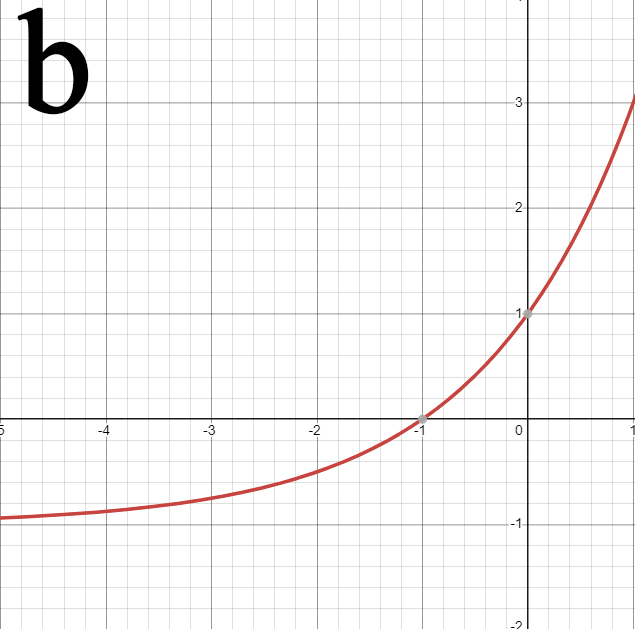
\includegraphics[width=0.25\textwidth]{grafic2.jpg}}
    \end{figure}
    \switchcolumn
    \begin{figure}[H]
        \hbox{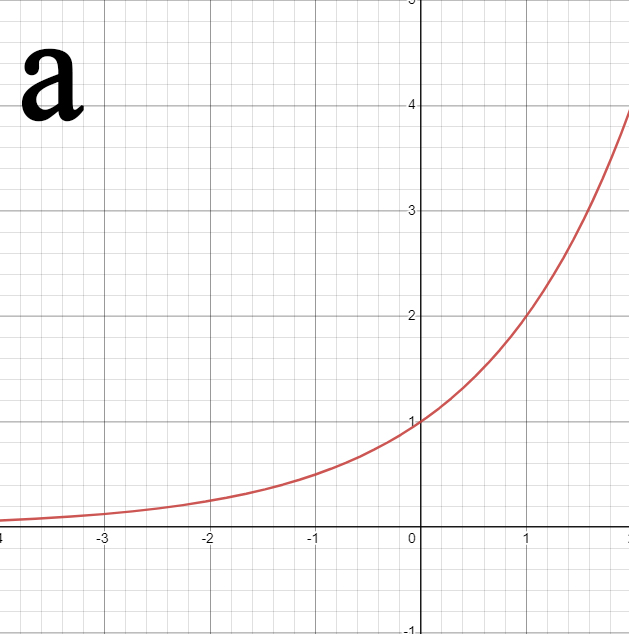
\includegraphics[width=0.25\textwidth]{grafic1.jpg}}
    \end{figure}
    \switchcolumn
    \begin{figure}[H]
        \hbox{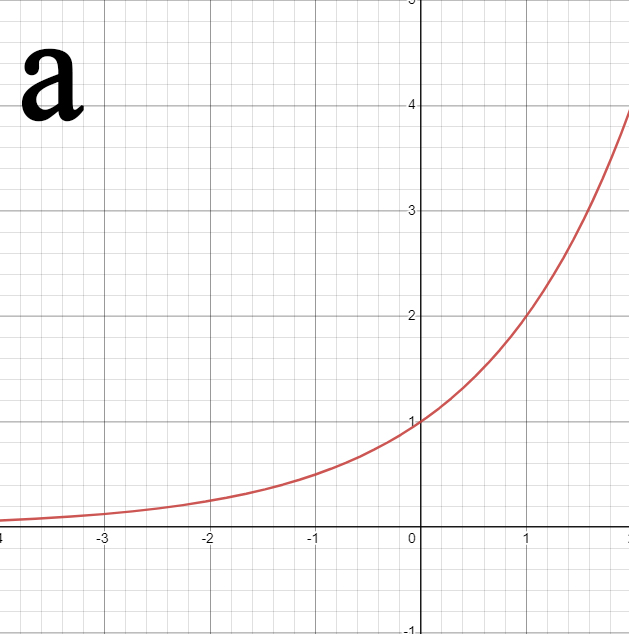
\includegraphics[width=0.25\textwidth]{grafic1.jpg}}
    \end{figure}
    \switchcolumn
    \begin{figure}[H]
        \hbox{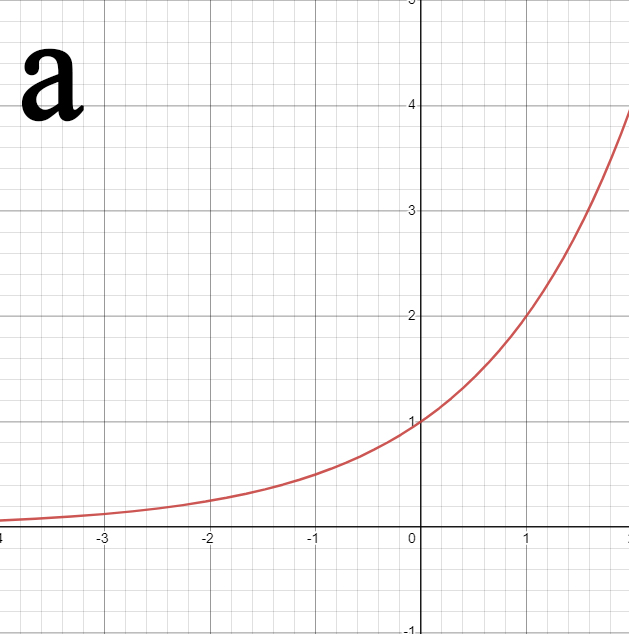
\includegraphics[width=0.25\textwidth]{grafic1.jpg}}
    \end{figure}
\end{paracol}

\end{document}